\section{Methods}
\label{sec:methods}
%Uma secao para cada tipo de sistema. Escrever descricao do problema e equacionamento. As baterias podem ser modeladas como uma fonte de calor.

%Justificar que apenas a condicao de voo sera considerada porque o aviao e de bater recorde, entao ele nao precisa ficar parado no sol

For the purposes of a preliminary design,
 the battery system of the aircraft is modelled as a simple stedy state heat exchange system.
The batteries are assumed to be an uniform heat source of constant power output.
The flight situation considered is leveled flight at full power on a warm day (ISA$+10$), normal day (ISA) and cold day (ISA$-10$).

In this section, the heat conduction models for the two proposed solutions for cooling the batteries are explained, as well as the model for determining the heat output of the batteries.

\subsection{The battery}
\label{sec:battery}
There are three types of batteries cells commonly used in the industry, such as cylindrical, prismatic and pouch cells. 

Cylindrical cell still is one of the most used packaging style due to its easiness of manufacture and good mechanical stability. It doesn't have an ideal stacking profile, but its higher energy density compensates for this flaw and the empty space can be used for cooling in order to improve thermal management.The cylindrical cell is commonly used in portable applications and is also used in Tesla electric vehicles.

Prismatic cells make optimal use of space by using the layered approach, allowing flexible design. In contrast, it can be more expensive to manufacture, less efficient in thermal management and have a shorter life cycle than its cylindrical counterpart. Usually encased in aluminum or steel for stability, small amount of swelling must be accounted for.

Pouch cells offer simple, flexible lightweight solutions to battery design. Makes most efficient use of space, achieving up to 95\% packaging efficiency, however, swelling allowances must be made. It is light and cost-effective.\cite{packaging}
%Elaborate on witch one will be used on the article (explain why --- was it a project choice? cost choice? or it is still not decided --- can we make comparisons?)

As a project decision, battery packs consisting of state-of-the-art Lithium Sulfur technology pouch cells, from Oxisenergy will be used. \Cref{fig:pouch} shows one of these pouches and \cref{fig:pack} shows an assembled pack.

\begin{figure}
    \centering
    \begin{subfigure}{0.45\textwidth}
    \includegraphics[width=0.9\textwidth]{fig/pouch.jpg}
    \caption{pouch}
    \label{fig:pouch}
    \end{subfigure}
    \begin{subfigure}{0.45\textwidth}
    \centering
    \includegraphics[width=0.9\textwidth]{fig/pack.jpg}
    \caption{pack}
    \label{fig:pack}
    \end{subfigure}
    \caption{Li-S battery by Oxys Energy}
\end{figure}

\subsection{Thermal model of the battery}
The heat generation per unit volume of the battery can be calculated from the internal resistance of each battery cell.This is a simplified model, which takes in consideration only Joule heat, disregarding polarization and reaction heat, which are known to occur in Li-S batteries.\cite{samba2015battery}

Considering a series arrangement%
\footnote{This is without loss of generality. Considering a parallel arrangement would lead to the same result}%
, the joule heating of the battery is given by 
\begin{equation}
\label{eqn:Q1}
\dot{Q} =  N R_i I^2
\end{equation}
where $N$ is the number of cells, $R_i$ is the internal resistance of each cell and $I$ is the current flowing through the cell. Denoted the voltage supplied by each cell as $V_\text{cell}$ and the power required by the engine as $P$, the electrical current is given by
\begin{equation}
\label{eqn:current}
    I = \frac{P}{N V_\text{cell}}
\end{equation}

Combining \cref{eqn:Q1} and \cref{eqn:current}, the heat dissipated by the battery $\dot{Q}$ is
\begin{equation}
\dot{Q} = \frac{R_i}{N} \frac{P^2}{V_\text{cell}^2}
\end{equation}

Finally, since the number of batteries is given by the ratio of battery mass to cell mass, i.e.
\begin{equation}
N = \frac{m_b}{m_\text{cell}}
\end{equation}
the total heat dissipated is
\begin{equation}
    \dot{Q}=R_i \frac{m_\text{cell}}{m_b} \frac{P^2}{V_\text{cell}^2}
\end{equation}


\subsection{Conduction cooling}
\label{sec:cc}
In order to minimize the airplane's weight and drag, it is ideal to cool the batteries passively by heat conduction through the airplane's skin. The batteries would be attached to the lower surface of the wing, in order to avoid radiation heating and maximize the area available for heat transfer.

The heat transfer problem that arises from this configuration is shown in \cref{fig:conduction}. Heat is generated uniformly in the batteries' pouches, which are insulated on one side and in contact with the wing's skin on the other. The heat is then conducted through the skin and transferred by convection to the air passing by the wing.

 \begin{figure}
     \centering
     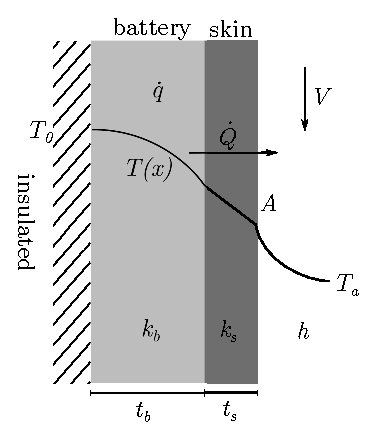
\includegraphics{fig/conduction.eps}
     \caption{Thermal system for conduction cooling}
     \label{fig:conduction}
 \end{figure}
 
 The equations that model this thermal system are
 \begin{align}
   T_0-T_{sb} &= \frac{\dot{q}}{2k_b}t_b^2 &\text{ for } 0 < x <t_b \\
   T_{sb}-T_{sa} &= \frac{\dot{Q}}{k_s A} t_s &\text{ for } t_b<x<t_b+t_s\\
   T_{sa} - T_a &= \frac{\dot{Q}}{hA} &\text{ for } x>t_b+t_s
 \end{align}
 where $T_0$ is the temperature at the insulated surface of the battery, $T_{sb}$ is the temperature at the battery-skin interface, $T_{sa}$ is the temperature at the skin-ambient interface and $T_a$ is the ambient temperature. $k_b$ and $k_s$ are the thermal conductivity of the battery and skin respectively, and $h$ is the convective coefficient of the air. $t_b$ and $t_s$ are the battery and skin thickness. $A$ is the surface area available for heat transfer, $\dot{Q}$ is the total heat flux generated by the battery, and $\dot{q}$ is the heat generated by unit of volume.
 
 Assuming uniform heat generation, i.e.\ $\dot{q} = \tfrac{Q}{At_b}$, these equations can be combined to relate the ambient temperature $T_a$ with the maximum temperature in the battery, $T_0$:
 \begin{equation}
    \label{eqn:conduction}
     T_0 = T_a + \frac{\dot{Q}}{A} \left(\frac{1}{h} + \frac{t_s}{k_s} + \frac{t_b}{2k_b} \right)
 \end{equation}
 
Alternatively, since the battery volume $\volume_b$ is known, the surface area can be expressed in terms of the battery thickness, i.e.\ $A = \frac{\volume_b}{t_b}$, or $Q/A = \dot{q} t_b$. Substituting this in \cref{eqn:conduction}, and doing some algebraic manipulation
\begin{equation}
    \frac{t_b^2}{2} + \left(\frac{k_b}{k_s} t_s + \frac{k_b}{h}\right) t_b - \frac{k_b}{\dot{q}}(T_0-T_a) = 0
\end{equation}

Solving for $t_b$ and choosing the positive root,
\begin{equation}
    t_b = t_s\left(\frac{k_b}{k_s} +\frac{k_b}{ht_s}\right)\left[\sqrt{1 + 2\left(\frac{k_b}{k_s} +\frac{k_b}{ht_s}\right)^{-2} \frac{T_0-T_a}{\dot{q}t_s}} - 1\right]
\end{equation}

The remaining step is to calculate the convection coefficient, $h$. For a high performance wing, a predominantly laminar boundary layer is expected. Kreith \cite{kreith} suggests the following relation for the local Nusselt number as a function of Reynolds and Prandtl numbers.
\begin{equation}
    Nu_x = 0.33\text{Re}_x^{1/2}\text{Pr}^{1/3}
\end{equation}
where the dimensionless coefficients are defined as follows
\begin{align}
\text{Nu} &= \frac{hx}{k} \\
\text{Re} &= \frac{\rho V x}{\mu} \\
\text{Pr} &= \frac{c_p \mu}{k}
\end{align}
$x$ is the chordwise dimension $k$ is the thermal conductivity, $\rho$ is air densisty, $V$ air speed, $c_p$ air specif heat at constant pressure, and $\mu$ is air's kinematic viscosity.

For getting a Nu valid for the entire wing, it is useful to consider $x=c/2$, where $c$ is the mean geometric chord. From Nu it is easy to calculate $h$.

\subsection{Air cooling}
\label{sec:air}
The most used system for cooling small aircraft generators and batteries is the air type. In this system, the battery pack is cooled by the stream of air forced through it by a pressure differential caused either by ram effect or a specially designed inlet, such as a NACA duct. In this subsection, the goal is to calculate the mass flow required for air cooling and the drag associated with it.

\begin{figure}
    \centering
    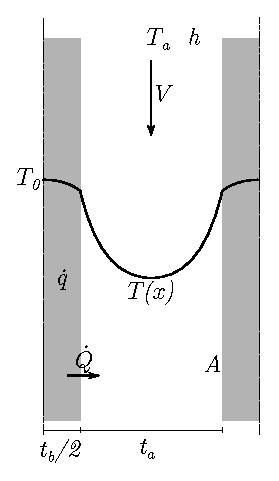
\includegraphics{fig/convection.eps}
    \caption{Thermal system for forced air convection cooling}
    \label{fig:convection}
\end{figure}

The thermal system for this case is shown in \cref{fig:convection}. In this schematic drawing, air is forced between two battery packs. The notation is the same that was followed in the previous section. Since the battery packs can be made relatively thin, the simplifying assumption that the temperature within the pack is uniform will be made.
The surface area $A$ can be calculated from the battery volume $\volume_b$ divided by $t_b/2$. The model is therefore governed by the equation
\begin{equation}
\dot{Q} = hA(T_0-T_a)
\end{equation}
From this we can calculate the Nusselt number
\begin{equation}
    \text{Nu} = \frac{h}{t_a k_a} = \frac{\dot{Q}}{t_a k_a A(T_0-T_a)}
\end{equation}
Kreith \cite{kreith} suggests the following relation between Nusselt and Reynolds for flow between parallel plates in electronic components:
\begin{equation}
    \text{Nu} = 0.093\text{Re}^{0.72}
\end{equation}
where the characteristic length for Re in $t_a$. Since $\text{Re} = \frac{\rho V t_a}{\mu}$, where $\rho$ is the density of the air and $\mu$ is the kinematic viscosity of air, the mass flow needed is given by
\begin{equation}
    \dot{m} = N (\rho V t_a h) = \text{height} \times N \mu \text{Re}
\end{equation}
where $N = \volume_b/\volume_\text{pack}$ is the number of battery packs.

Finally, the drag can be calculated considered a ram inlet, and is
\begin{equation}
    D = \tfrac{1}{2}\rho V_\infty^2A_\text{inlet} = \tfrac{1}{2} \dot{m}V_\infty
\end{equation}
where $V_\infty$ is the speed of flight and $A_\text{inlet}$ is the inlet area.

%Por motivos obvios (tempo) nao existe water cooling
%\subsection{Water cooling}
%
%Conveccao forcada de agua e um radiador. Para esse caso precisamos estimar o peso do sistema, a vazao massica de ar necessaria para o radiador e o arrasto da entrada de ar. Isso para manter as baterias a uma temperatura pre estabelecida